\documentclass[10pt]{article}
\usepackage[margin=0.9in]{geometry}
\usepackage{amsmath,amssymb,booktabs,graphicx,microtype,natbib,hyperref,tikz}
\hypersetup{hidelinks}
\usetikzlibrary{arrows.meta,positioning}
\graphicspath{{figures/}}
\title{Evaluating Oversight in Sequential Commons}
\author{Ameer Alhashemi}
\date{Working draft: 24 September 2026}
\begin{document}
\maketitle
\begin{abstract}
Agents drawing from a shared resource can satisfy individual rules while the resource becomes unsafe. We study how much information a reviewer needs to distinguish harmful joint requests from safe ones without suppressing useful extraction. Earlier Harvest experiments motivate the question; a matched comparison gives reviewers the same one-step safety target and intervention menu, and varies how many current requests they inspect. In two pilot-selected Fishery and Harvest settings, joint review restricts fewer safe requests than a deliberately conservative local rule without approving more requests classified as risky. A post-hoc replay shows that a local calculation using inspected neighbouring contributions exactly matches joint decisions on the saved proposals. Thus the observed gap concerns the information discarded by a particular local rule, not an inherent advantage of central review. Immediate decision quality also need not predict long-run return. These two settings form a controlled study of oversight information, not a validated actor--overseer capability scale or a general multi-game benchmark.
\end{abstract}

\section{Problem and Research Question}
Consider several agents drawing from a resource that replenishes over time. Each agent benefits from extraction, but its action can reduce future supply or damage neighbouring resources. A monitor may inspect requests, announce limits, or restrict extraction. We ask:
\begin{quote}
When reviewers have limited access to agents' current requests, what information is needed to reject harmful joint use while retaining safe activity?
\end{quote}
A local rule and a global safety condition can disagree for several reasons. An acceptable request can occur after damage has already accumulated. Weather can worsen the resource after an action. Neighbours' simultaneous requests can also matter. The benchmark must distinguish these explanations rather than treating every disagreement as evidence that local oversight cannot work.

Scalable oversight motivates this question: supervision becomes difficult when relevant behaviour exceeds the overseer's information, judgment, or ability to intervene. We study a restricted part of that problem through inspectable policies and fixed mechanisms. Search budget and intervention limits are separate factors. We do not measure a general intelligence gap between a trained actor and a trained verifier.

Our contribution is a matched oversight protocol and diagnostic controls in two sequential commons games. We measure harmful approvals, safe requests restricted, monitoring effort, and resource outcomes separately. The current evidence concerns these specified policy populations and known transition rules; it does not demonstrate a general capability gap or compare deployable oversight institutions.

\section{Background and Scope}
Sequential social dilemmas concern cooperation across policies and repeated interaction rather than a single cooperate/defect action \citep{leibo2017sequential}. Melting Pot and SocialJax provide broader environments and evaluation infrastructure \citep{agapiou2022meltingpot,guo2025socialjax}. Our small numerical implementation follows this problem family; it is not an implementation or performance competitor of those suites.

Commons scholarship motivates examining rules, monitoring, incentives, and institutional fit \citep{ostrom1990governing}. It does not validate this simulator's numerical settings. Multi-agent shielding studies intervention on joint actions and factored safety mechanisms \citep{elsayedaly2021shielding}. Contract-based shielding shows how coordinated local obligations can preserve safe joint behaviour without centralized runtime control \citep{adalat2026contracts}. Studies of distributed attacks and monitoring likewise show that individually benign-looking steps can combine into harmful outcomes \citep{hu2026compositional,makins2026multiagent}. Neither local/global disagreement nor distributed review is our novelty claim. Our filters have no formal shield guarantee. We instead measure the safety--activity cost of specific information and aggregation choices in renewable-resource dynamics.

Scalable-oversight benchmarks operationalize supervision on defined tasks \citep{bowman2022scalable,sudhir2025benchmark}. \citet{engels2025scaling} estimate oversight-specific performance across actor/overseer pairings. Subtracting our assigned generation and intervention ranks would not inherit that measurement justification. We therefore retain their separate settings.

GovSim already studies resource-use language-model societies, communication, and sustainability \citep{piatti2024govsim}. Related work generates complete strategies and studies their interactions or spread through populations \citep{willis2025cooperate,willis2026hundreds}. Our model-policy experiment adopts the offline strategy interface. Its additional control tests what model generation contributes beyond numerical policy suggestions in the prompt.

\paragraph{Why Fishery and Harvest?}
Fishery has one renewable stock, so the effect of adding several harvest requests is directly visible. Harvest adds local patches, neighbour spillovers, messages, and optional transfers. The population and mechanism studies use Harvest. A later matched-information comparison uses both games with the same reviewer rules but game-specific safety conditions; their returns are not pooled. Earlier Fishery and PPO work remains supporting evidence under different protocols.

The Harvest settings retain internal names \texttt{community\_irrigation} and \texttt{forest\_co\_management} for reproducibility. We call them moderate and high stress. They change regeneration, externalities, population composition, and other parameters. They are not field-calibrated agricultural or forestry models, and comparing them does not isolate coupling alone.

\section{Game and Evaluation Protocol}
\subsection{Players and decisions}
There are $n$ resource users. The finite-horizon, general-sum game has augmented state
\[
s_t=(\mathbf x_t,\mathbf v_t,\mathbf p_{t-1},z_t),
\]
where $\mathbf x_t$ contains patch resources, $\mathbf v_t$ contains credit-related memory, and $z_t$ includes time, the governor's trend history, pending interventions, and failure streak. This augmentation accounts for history-dependent intervention and termination.

User $i$ has policy parameters $\phi_i$ supplied by a generator $\mathcal G_b$ with settings $b$. Its observation contains local resource, neighbour mean resource, previous credit received, and any announced cap. Neighbour resource information is present even when messaging is disabled. The policy chooses a harvest request $p_{i,t}\in[0,1]$ and an optional transfer offer $u_{i,t}$. The structured policy class specifies resource thresholds, harvest fractions, reciprocity, and cap responses.

The governor is a fixed stateful rule, not a trained strategic player. It observes exact mean resource and previous requests, then announces caps using resource and trend triggers. Users can respond before enforcement. An intervention map produces allowed fractions:
\[
\mathbf a_t=I_{m,\ell}(s_t,\mathbf p_t;\zeta_t),\qquad
s_{t+1}\sim P_{\theta,m,\ell}(\,\cdot\mid s_t,\mathbf p_t,\mathbf u_t,\zeta_t).
\]
Here $\theta$ specifies environment dynamics, $m$ the mechanism, $\ell$ its limits, and $\zeta_t$ any randomized enforcement decisions. The transition includes the intervention map, resource dynamics below, and credit and monitor-memory updates. The experimenter chooses the settings. We evaluate trajectories rather than solve an equilibrium among optimizing overseers and users.

Figure~\ref{fig:reviewer-interface} previews the later matched-reviewer
experiment; it does not depict every announcement and transfer in the
historical governance packages.

\begin{figure}[t]
\centering
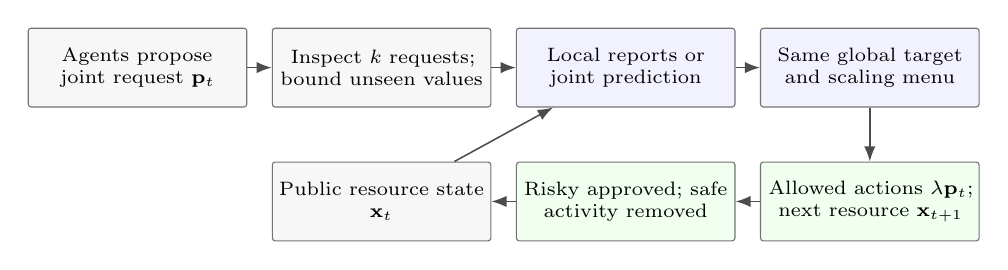
\begin{tikzpicture}[font=\scriptsize,>=Latex,
  box/.style={draw=black!55,rounded corners=1pt,align=center,
    minimum height=10mm,inner sep=2.5pt,text width=26mm},
  flow/.style={->,line width=.55pt,draw=black!70}]
\node[box,fill=black!3] (requests) at (0,0)
  {Agents propose\\joint request $\mathbf p_t$};
\node[box,fill=black!3] (view) at (3.1,0)
  {Inspect $k$ requests;\\bound unseen values};
\node[box,fill=blue!5] (predict) at (6.2,0)
  {Local reports or\\joint prediction};
\node[box,fill=blue!5] (choice) at (9.3,0)
  {Same global target\\and scaling menu};
\node[box,fill=black!3] (state) at (3.1,-1.7)
  {Public resource state\\$\mathbf x_t$};
\node[box,fill=green!6] (readout) at (6.2,-1.7)
  {Risky approved; safe\\activity removed};
\node[box,fill=green!6] (transition) at (9.3,-1.7)
  {Allowed actions $\lambda\mathbf p_t$;\\next resource $\mathbf x_{t+1}$};
\draw[flow] (requests)--(view);
\draw[flow] (view)--(predict);
\draw[flow] (state)--(predict);
\draw[flow] (predict)--(choice);
\draw[flow] (choice)--(transition);
\draw[flow] (transition)--(readout);
\draw[flow] (readout)--(state);
\end{tikzpicture}
\caption{Matched reviewer interface. Agents' requests and the public resource state enter a limited inspection view; reviewers differ in their prediction calculation, not in the global safety target or available uniform scaling actions. Risky approvals and safe restrictions are evaluated on the original proposal, while resource outcomes come from the executed action.}
\label{fig:reviewer-interface}
\end{figure}

\subsection{Resource dynamics and payoffs}
Let $M$ be maximum extraction and $K$ patch capacity. Actual harvest is $h_{i,t}=\min(Ma_{i,t},x_{i,t})$. Excess above the reference fraction $\alpha$ is $e_{i,t}=[h_{i,t}-M\alpha]_+$. For neighbours $\mathcal N_i$,
\begin{align}
y_{i,t}&=\left[x_{i,t}-h_{i,t}-\eta\sum_{j\in\mathcal N_i}e_{j,t}\right]_+,\\
x_{i,t+1}&=\operatorname{clip}_{[0,K]}
\left(y_{i,t}+[r y_{i,t}(1-y_{i,t}/K)]_+ + \xi_{i,t}\right).
\end{align}
Here $r$ is regeneration, $\eta$ spillover strength, and $\xi_{i,t}$ Gaussian weather noise. The code's sustainable-harvest parameter is a nominal reference, not a guarantee under every setting.

User payoff is harvest plus received transfers, minus outgoing transfers and charged intervention cost. The historical governor deducts price $\beta$ from targeted users and also logs it as burden. Burden must not be subtracted from net welfare twice. New mechanism checks disable transfers and set monetary intervention price to zero, reporting prevented extraction, intervention incidence, and returns.

\subsection{Generation and intervention settings}
The initial low setting uses mutation. The other settings select among six candidates evaluated for 30 steps or twelve evaluated for 60 steps. Search maximizes entrant episode payoff minus a 25-point collapse penalty. Policies are selected and replaced between generations, while each evaluation episode resets. Additional search is a resource allocation whose benefit requires independent validation.

Historical oversight presets bundle target-selection recall $q$, delay $d$, target share $\kappa$, and price $\beta$. Recall acts during enforcement; it does not degrade the governor's aggregate observation. Price does not impose an exhaustible budget. With six agents, the historical rounding rule permits one target at share 0.33 and at least one even at zero share. New checks explicitly use floor rounding, including zero targets at zero capacity. Historical results remain unchanged.

The original local-only package enables communication and optional transfers without a system-level governor. Global-only uses uniform cap targeting without those channels. Hybrid enables communication and changes to neighbourhood targeting with neighbour expansion. The original comparison therefore evaluates packages, including populations selected under each package. It does not isolate communication or targeting.

\subsection{Safety diagnostics}
For requested fractions define
\[
L_{i,t}^{\epsilon}=\mathbf1[p_{i,t}\leq\alpha+\epsilon],
\quad A_t=\prod_i L_{i,t}^{\epsilon},
\quad G_t^{\tau,\rho}=\mathbf1[\bar x_t\geq\tau\ \land\ f_t<\rho],
\]
where $\bar x_t$ is mean resource and $f_t$ is the fraction below the patch-failure threshold. Local-pass/global-fail is
\[
F_t=A_t(1-G_{t+1}),\qquad
\mathrm{LPGF}=\frac1D\sum_{t=0}^{D-1}F_t,
\]
with executed duration $D\leq T$, including early termination. This is unsafe occupancy during local approval. It does not by itself show that approved actions caused failure.

We separately record
\[
O_t=G_tA_t(1-G_{t+1}),\qquad
P_t=(1-G_t)A_t(1-G_{t+1}),
\]
for approved onset and persistence. Coverage is $\sum_tA_t/D$; conditional unsafe occupancy is $\sum_tF_t/\sum_tA_t$, unavailable when no steps pass. Reports include all four local/global outcomes.

After intervention, allowed fractions $\mathbf a_t$ receive a separate check. A clean-prefix onset requires every allowed action up to that onset to have passed the fixed cutoff. State-based filters additionally have their own predicted-local-state check; this differs from the fixed fraction predicate. Outcomes include health, total and per-step net return, duration, and removed requests $M\sum_i(p_{i,t}-a_{i,t})$. The latter is nominal requested extraction, not necessarily harvest that would have been available. Winner counts cannot substitute for these quantities.

\paragraph{Development evidence.}
An earlier Harvest package sweep identified a local/global mismatch, but its
packages change several factors together and its scalar capability-gap rank
collapses distinct treatments. It motivates the matched checks below rather
than providing an architecture ranking. The full descriptive results and
threshold-replay caveat are in Appendix~\ref{app:population-study}.

\section{Matched Checks}
\subsection{Protocol}
We restore twenty final-generation no-governor populations: five runs for each stress setting and low/high generation process. All 120 agent positions are verified against the original per-agent archive. Eight new weather seeds per population are shared across mechanisms.

The controls are no intervention; messages alone; messages on/off crossed with uniform/neighbourhood targeting; a fixed cutoff filter; a local state filter; announcement without enforcement; and a joint-action reference. Transfers are disabled. Cap packages use $q=0.7$, $d=1$, $\kappa=0.5$, and $\beta=0$. The filters have full filtering authority; they are diagnostic references rather than equal-capacity alternatives.

The fixed filter enforces $\alpha+\epsilon$. The local state filter predicts own-patch regrowth with zero weather and no knowledge of neighbours' current requests, restricting harvest so its prediction remains at least 10. The joint reference predicts all patches from full current requests, including spillovers, and scales joint extraction until predicted global safety passes. Both are one-step models without a weather uncertainty allowance. A $10^{-8}$ numerical buffer avoids rounding below the boundary. Infeasible states remain in the analysis.

The base screen contains 3,520 episodes, including removal of weather, spillovers, or both for no intervention and the three filters. Because failures are sparse in the base screen, we repeat the unchanged protocol under the already-defined slow-regrowth regime, adding 3,520 episodes. This evidence-guided follow-up is exploratory; neither the base result nor its thresholds are replaced.

Uncertainty uses source-run means after averaging weather seeds. Deterministic no-weather repeats do not provide independent evidence. Search calibration separately uses twelve fresh parent/opponent contexts per setting, nested candidate counts 1/6/12, crossed 30/60-step selection horizons, and sixteen unseen test seeds at horizon 80. Its 2,304 held-out episodes test performance independently of candidate selection.

\subsection{Local checks and resource failure}
\begin{table}[t]\centering\small
\begin{tabular}{lrrrr}\toprule
& \multicolumn{2}{c}{Base regrowth} & \multicolumn{2}{c}{Slower regrowth}\\
Mechanism & Moderate & High & Moderate & High\\\midrule
None & 0.00 & 0.81 & 1.53 & 19.70 \\
Messages only & 0.00 & 0.00 & 0.66 & 0.00 \\
Announcement only & 0.00 & 0.00 & 0.00 & 0.00 \\
Uniform caps & 0.00 & 0.00 & 0.00 & 0.00 \\
Neighbourhood caps + messages & 0.00 & 0.00 & 0.00 & 0.00 \\
Fixed local filter & 0.00 & 0.00 & 0.00 & 5.33 \\
Local state filter & 0.00 & 0.02 & 0.00 & 0.12 \\
Joint reference & 0.00 & 0.61 & 0.66 & 8.30 \\
\bottomrule\end{tabular}
\caption{Unsafe step percentages in matched-policy checks. Each cell has ten fixed populations (five source runs at each generation treatment) and eight seeds. These are descriptive means; generation treatment and source-run variation are retained in the accompanying data. The slow-regrowth follow-up uses an existing held-out condition.}
\label{tab:matched}\end{table}

In the base screen, the fixed filter has no globally unsafe steps. Final-generation populations are often stable already: without intervention, unsafe occupancy is zero in moderate stress and 0.81\% in high stress. The local state filter records one predicted-local-pass/global-onset event with weather and spillovers; it is absent in the corresponding removal controls. This single event supports no general claim.

Under slower regrowth in high stress, no intervention has 19.70\% unsafe occupancy and the fixed filter has 5.33\%. Sixteen of eighty fixed-filter episodes have an unsafe onset while all allowed actions have passed the cutoff throughout. Removing weather still leaves a failure for one of the ten fixed populations; eight deterministic seed repeats reproduce that same case. Removing both weather and spillovers eliminates those onsets. Thus the fixed cutoff can miss failure from accumulated resource use and spillovers, even without a previous rule violation. The result concerns this cutoff and these dynamics, not every possible local rule.

The local state filter reduces slow-regrowth/high-stress unsafe occupancy to 0.125\%. It has eight predicted-local-pass onset steps across six episodes when both weather and spillovers are present, and none in their removal controls. A more informative local check is therefore a strong baseline, not a mechanism the benchmark can assume to be inadequate.

The joint reference has 8.30\% unsafe occupancy in that same condition. It permits actions near the mean-health boundary under a zero-weather prediction, and it enforces a different condition from maintaining every predicted local patch above 10. This comparison does not isolate the value of global information. It shows why prediction assumptions, safety objectives, and reserve margins must be matched before claiming an information advantage.

Safety improvements need not reduce return. In this condition, the local state filter increases mean health from 11.12 to 11.79 and total population return from 980.48 to 1,028.95 relative to no intervention. Uniform caps maintain higher health, 14.74, with lower return, 908.18. These descriptive comparisons show why resource protection and productive use must both be reported; monetary intervention cost is zero throughout this check.

\begin{figure}[t]
\centering
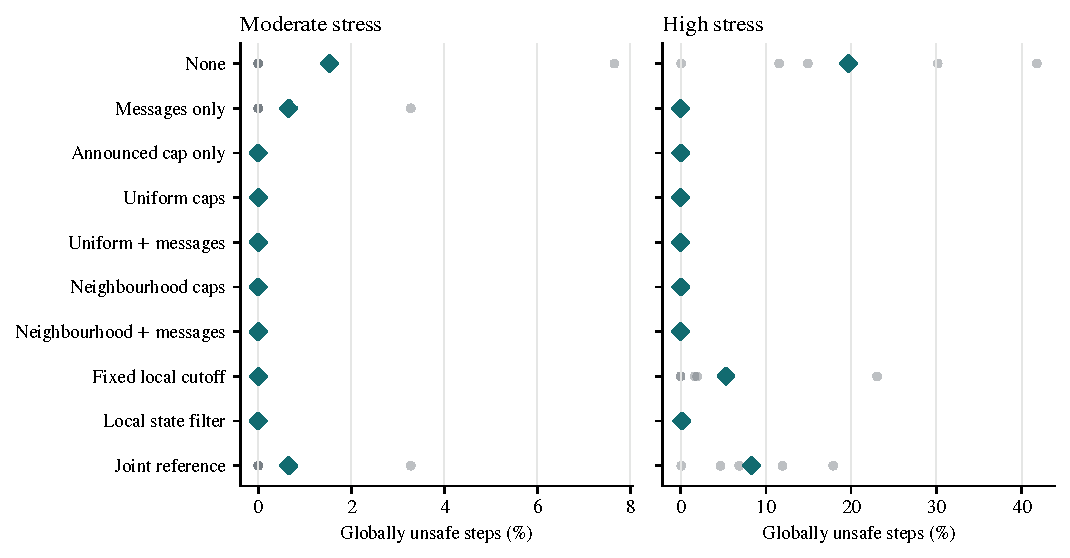
\includegraphics[width=.97\linewidth]{matched_mechanisms_slow}
\caption{Frozen-policy results under the existing slow-regrowth regime. Diamonds are means; dots are five source-run averages after averaging generation treatments and seeds. The state-aware local filter sharply reduces unsafe occupancy relative to the fixed cutoff. The joint reference uses a different, zero-weather global prediction and is not a guaranteed-safe oracle.}
\end{figure}

\subsection{Announcements, enforcement, and search}
Announcement alone produces no globally unsafe steps in both the base and slow-regrowth screens. The policies explicitly respond to announced caps, so some protection occurs before enforced clipping. In the base screen, adding uniform enforcement reduces total return relative to announcement alone by 11.45--39.07 across setting/generation cells. These are policy-class-specific results, not evidence that announcements will constrain arbitrary agents.

\begin{figure}[t]
\centering
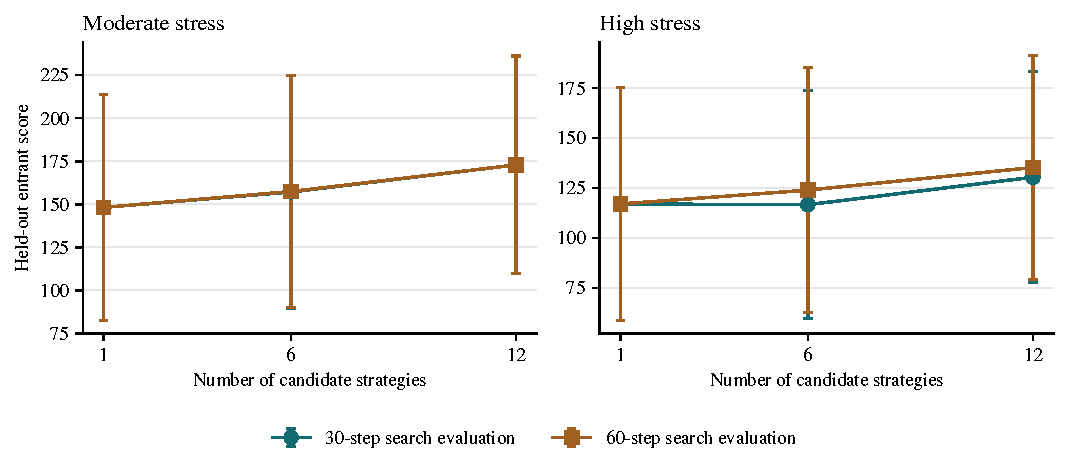
\includegraphics[width=.97\linewidth]{generator_validation}
\caption{Generator quality on unseen episodes. Score is entrant payoff minus the predefined collapse penalty. Error bars are nominal 95\% $t$ intervals across twelve parent contexts, without multiple-comparison correction. Candidate count and selection horizon remain separate factors.}
\end{figure}

In moderate stress, six-candidate selection improves held-out score over one candidate by 8.98 (95\% interval 2.51--15.44) at a 30-step search horizon and 9.23 (2.70--15.77) at 60 steps. Twelve-candidate point estimates are higher but uncertain. In high stress, all score-difference intervals include zero. These exploratory results support some within-setting search benefit, not a reliable low/medium/high ordering across settings. Resource damage is reported separately from the optimization objective.

\section{Limited-Inspection Reviewers}
The previous joint-action reference and local filter had different prediction
targets and uncertainty assumptions. To isolate the role of current-request
information, we now compare three reviewers with the same one-step global
safety target and the same intervention authority. Each can multiply the
whole proposed request vector by one of $1,0.75,0.5,0.25,0$ and evaluate at
most five candidates. A joint reviewer accounts for all visible requests
together. A bounded local reviewer predicts from individual reports while
conservatively bounding unseen neighbour extraction; its reports are pooled
before a global decision. An optimistic local reviewer omits neighbour
extraction. The latter is a useful activity-preserving comparator, not a
guaranteed-safe method. All methods have the same public resource state,
inspect the same nested subset of zero, three, or six requests, and bound
uninspected requests by one. Harvest predictions use the same weather margin.
None sees the future disturbance or the reference label.

We selected two settings for two-class coverage using the preceding development
pilot: Fishery with four aggressive policies and Harvest with two under slower
renewal. Sixty-four fresh population contexts per game supply original joint
requests from no-intervention episodes. Each request is tested under every
reviewer and inspection budget. The one-step reference is exact in Fishery; in
Harvest it is a 128-draw Monte Carlo risk estimate with a 0.05 threshold and
Wilson intervals. Ambiguous Harvest cases are labelled unresolved, not safe.
The resulting 1,920 episodes contain 694 resolved-safe and 63 resolved-risky
Fishery requests from initially safe states, and 3,687 safe, 1,368 risky, and
923 unresolved Harvest requests. Contexts, rather than repeated requests or
weather streams, are the independent units.

\begin{table}[t]
\centering\small
\begin{tabular}{llrr}
\toprule
Setting, six inspected & Reviewer & Risky approved & Safe restricted \\
\midrule
Fishery & Joint & 0/63 & 0/694 \\
 & Bounded local & 0/63 & 100/694 \\
 & Optimistic local & 63/63 & 0/694 \\
\addlinespace
Harvest & Joint & 0/1,368 & 2,521/3,687 \\
 & Bounded local & 0/1,368 & 3,687/3,687 \\
 & Optimistic local & 0/1,368 & 2,407/3,687 \\
\bottomrule
\end{tabular}
\caption{Matched decisions on fresh original joint requests from initially
safe states. ``Restricted'' means the original request was scaled down,
possibly partially, not that all extraction stopped. The Harvest setting does
not distinguish reviewers on risky approvals; the optimistic local rule
retains slightly more safe activity than joint review.}
\label{tab:budgeted-review}
\end{table}

\begin{figure}[t]
\centering
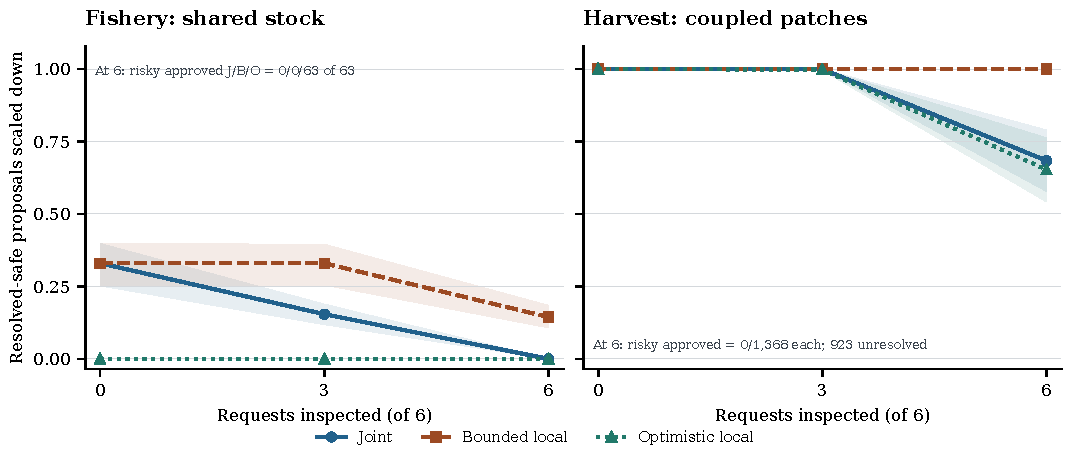
\includegraphics[width=\linewidth]{fig08_reviewer_decisions}
\caption{Safe original joint requests scaled down as inspection increases, on the fresh confirmation cohort. Lines are fractions of resolved-safe requests; shading shows 95\% bootstrap intervals resampling the 64 independent population contexts in each game. All methods use the same one-step safety target and scaling options. At full inspection, Fishery's optimistic local rule accepts all 63 resolved-risky requests; the others accept none. In Harvest no method accepts any of 1,368 resolved-risky requests in this selected setting, while 923 reference labels remain unresolved. Restriction can mean partial scaling, not complete loss of activity.}
\label{fig:reviewer-decisions}
\end{figure}

At six inspections, joint review restricts 14.4 percentage points fewer
resolved-safe Fishery requests than bounded local review (95\% bootstrap
interval over population contexts: 10.9--18.6 points fewer). In Harvest the
difference is 31.6 points fewer (21.1--41.7). Neither method approves a
resolved-risky request in either selected setting. Optimistic local review
approves all 63 resolved-risky Fishery requests, but none of Harvest's 1,368;
in Harvest it restricts 3.1 points fewer safe requests than joint review
(2.3--4.1). Thus the value of the current joint calculation relative to these
two local approximations depends on the resource dynamics and the chosen
approximation. Figure~\ref{fig:reviewer-decisions} shows that several Harvest
comparisons are saturated at low inspection budgets. Zero observed risky
approvals, or a degenerate bootstrap interval when paired methods agree, does
not establish zero underlying risk.

\paragraph{Coupled local diagnostic.}
After inspecting this result, we added a stronger local calculation that uses
the same inspected requests as joint review. Fishery aggregates bounded
per-user extraction contributions; each Harvest patch report includes the
two neighbouring excess-extraction contributions. Uninspected requests retain
the same upper bound, and the global predicate and action menu are unchanged.
The resulting calculation is algebraically equivalent to joint prediction.
In a post-hoc replay of all 11,249 saved proposals at three inspection budgets
(33,747 paired decisions), its selected scale, verdict, and status agree with
joint review in every case. This is an implementation check and a boundary on
the earlier contrast, not an independent empirical confirmation. It assumes
truthful sharing and a known transition model; its logical scalar report count
is higher than the joint reviewer's in the present accounting. The experiment
does not show an intrinsic advantage of central over sufficiently informed
distributed calculation.

\paragraph{An illustrative original request.}
In Fishery context 0, step 14, the stock is 21.21 and the six requested
fractions are $(0.568,0.092,0.574,0.558,0.159,0.499)$. All six requests are
inspected. Their actual combined demand is 14.70 units, and the exact
one-step prediction leaves stock at 10.77, above the safety cutoff of 10;
the joint reviewer approves the original request. The coarse bounded local
rule instead substitutes six times the largest individual request, a demand
bound of 20.65. At its available scales of 1 and 0.75, this predicts stock
below 10, so it chooses 0.5. This saved example explains one unnecessary
restriction: the information was available, but the bound discarded how the
six contributions differed. It is a mechanism illustration, not a separate
effect estimate.

The complete trajectories further distinguish immediate decisions from
long-run outcomes. At six inspections, Fishery joint review returns 551.5
over 80 steps on average versus 784.7 under bounded local review, despite
restricting fewer originally safe requests; its mean stock is 16.88 versus
25.58. More present extraction leaves less future stock. Both have zero
fixed-horizon unsafe fraction in this sample. In Harvest all three monitored
reviewers have zero unsafe fraction in this setting, so that outcome cannot
rank them. No-intervention fractions are 0.864 in Fishery and 0.421 in Harvest,
under an absorbing-failure convention. These are conditional comparisons of
known-transition reviewers, not evidence that a generally stronger actor was
supervised by a weaker learned overseer.

\begin{table}[t]
\centering\small
\begin{tabular}{llrr}
\toprule
Setting & Joint minus & Total return & Mean resource health\\
\midrule
Fishery & Bounded local & $-233.2\;[-259.8,-207.6]$ & $-8.70\;[-9.76,-7.69]$\\
Fishery & Optimistic local & $330.2\;[316.8,339.8]$ & $-9.35\;[-10.01,-8.60]$\\
Harvest & Bounded local & $28.1\;[15.7,38.8]$ & $-0.75\;[-0.80,-0.71]$\\
Harvest & Optimistic local & $0.5\;[-1.0,2.5]$ & $0.04\;[0.037,0.050]$\\
\bottomrule
\end{tabular}
\caption{Paired long-run differences at six inspected requests; brackets give 95\% percentile bootstrap intervals over 64 independent population contexts per game, averaging weather seeds within context. Negative Fishery stock and return differences against bounded local show that sparing a presently safe request need not improve renewable-resource outcomes. These are selected settings, not game-family averages.}
\label{tab:longrun-paired}
\end{table}

\section{Saved Model Policies and a Direct-Sampler Control}
Qwen 2.5 3B and Llama 3.2 3B each supplied 32 cooperative and 32 exploitative structured policies offline \citep{yang2024qwen25,meta2024llama32}. Parsing, bounds checks, clamping, and exact deduplication make reusable artifacts. They do not establish policy discovery or behavioural diversity.

The prompt supplies numerical anchors for all fourteen policy fields, drawn from separate ranges for cooperative and exploitative behaviour. Qwen reproduces all anchors in 35 of 64 policies; Llama does so in two. We compare saved policies against policies made directly from those anchors, using the same sampled indices, positions, and weather seeds. The control has two settings, three mixtures, no intervention/uniform caps, eight sampled populations, and four seeds: 1,536 episodes without new model calls.

At fully exploitative composition, both saved-model and anchor-only populations collapse in every tested no-intervention cell; neither collapses under uniform caps. Numerical outcomes differ, but the broad pattern does not require a language model. The supported claim is compatibility with model-produced policy artifacts. Additional models would not resolve this attribution issue. Comparisons are conditional on these fixed banks and this prompt design, not estimates of model-family performance.

\section{Limitations and Next Steps}
This benchmark remains exploratory. It does not establish a general actor--overseer capability scale, a universal failure of local enforcement, or a universally superior architecture. The original architecture study combines adaptation and intervention; the frozen-policy screens cover only twenty selected populations. Weather seeds and repeated thresholds do not replace independent populations.

Global unsafe occupancy, resource health, total return, and intervention burden answer different questions. Early termination affects historical per-step averages. New logs retain totals and duration; any future absorbing-failure or fixed-horizon return convention must be defined in advance.

The limited-inspection comparison addresses the earlier mismatch in safety targets and intervention authority, but only in two pilot-selected settings with known transition rules. A full-information reviewer using those rules is a diagnostic reference, not a deployable learned overseer. Equal request-inspection budgets do not imply equal total model checks or communication; both are logged separately. The coupled-local replay shows that the original bounded local rule discards useful inspected information. Its report-count comparison is a logical accounting model, not measured latency or a strategic communication experiment. The primary decision metric marks any scaling of a safe original request as restriction; it does not measure the amount retained. A post-hoc diagnostic from saved decisions separates partial scaling from complete stoppage, but requires prospective uncertainty analysis before it becomes a primary claim. The Fishery and Harvest samples are not interchangeable game-family replicates. A separate study would need to validate rising actor strategy-generation resources against the same reviewer protocol to connect this information result to capability pressure. Adding live language-model agents or more games would not by itself establish that link.

A benchmark release also requires accessible data, configurations, source hashes, dependencies, and a small reproducible example. Atomic result blocks, source-run-aware summaries, and manifests are implemented; complete external reproduction remains a release task. Earlier Fishery, PPO, institutional-friction, and model-policy work remains available as supporting evidence rather than being merged into one unqualified claim.

\section{Conclusion}
The study separates rule compliance, failure onset, persistent risk, and intervention effects in sequential commons. A fixed local cutoff fails in some slow-regrowth conditions, while a state-based local rule is a strong control. With a matched one-step target and action menu, the tested joint calculation spares safe activity relative to a coarse conservative local rule. Once local reports include the inspected coupled contributions, they reproduce its decisions on saved proposals. This shifts the question from whether oversight is centralized to what information must be shared, at what cost, and with what effect on long-run resource use. Those costs and strategic reporting remain open; increasing actor capability requires a separate matched test.

\bibliographystyle{plainnat}
\bibliography{refs}
\clearpage
\appendix
\section{Earlier Population Study}\label{app:population-study}
Stage A contains 360 run rows: two stress settings, three generation settings, three oversight presets, four packages, and five runs per cell. Each has six users and 15 generations, with 32 training seeds and 32 test seeds in each of four held-out regimes per generation. The following averages combine generations and test regimes.

\begin{table}[h]
\centering\small
\begin{tabular}{lrrrrr}
\toprule
Package & Unsafe (\%) & LPGF (\%) & Health & Return/step & Burden/episode\\
\midrule
None & 19.41 & 2.06 & 11.42 & 14.75 & 0.00\\
Local coordination & 13.92 & 1.18 & 11.62 & 14.68 & 0.00\\
Uniform-cap package & 6.13 & 2.35 & 14.22 & 12.34 & 2.10\\
Hybrid package & 4.10 & 1.24 & 14.33 & 12.52 & 2.05\\
\bottomrule
\end{tabular}
\caption{Descriptive Stage A averages. Cap packages preserve more resource on average but reduce per-step net return. Inactive-overseer copies for none/local do not supply independent replicates. LPGF orders the packages differently from resource health.}
\end{table}

The comparisons establish package-level differences. They combine direct intervention and the populations selected under that intervention. Slow regrowth produces the largest mean unsafe rate without oversight, 28.31\%, compared with 15.90--16.88\% in the other held-out regimes.

The earlier scalar gap combined distinct treatments. Low generation with weak oversight and high generation with strong oversight both receive gap zero, but their high-stress hybrid unsafe rates are 9.15\% and approximately zero. We retain separate factors in the supplementary plot. None/local outcomes are exactly invariant to the unused overseer presets.

The completed threshold replay contains 9,000 rows across 25 cutoff pairs. Resource health, return, and burden are identical within the same underlying run across those pairs: the cutoffs relabel trajectories rather than change intervention. This supports diagnostic sensitivity analysis, not additional independent resource-protection replications. The archived illustrative case contains 29 LPGF steps, all following an already-unsafe state; it supports persistence, not approved onset.

\section{Separate Generation and Oversight Factors}
\begin{figure}[!ht]
\centering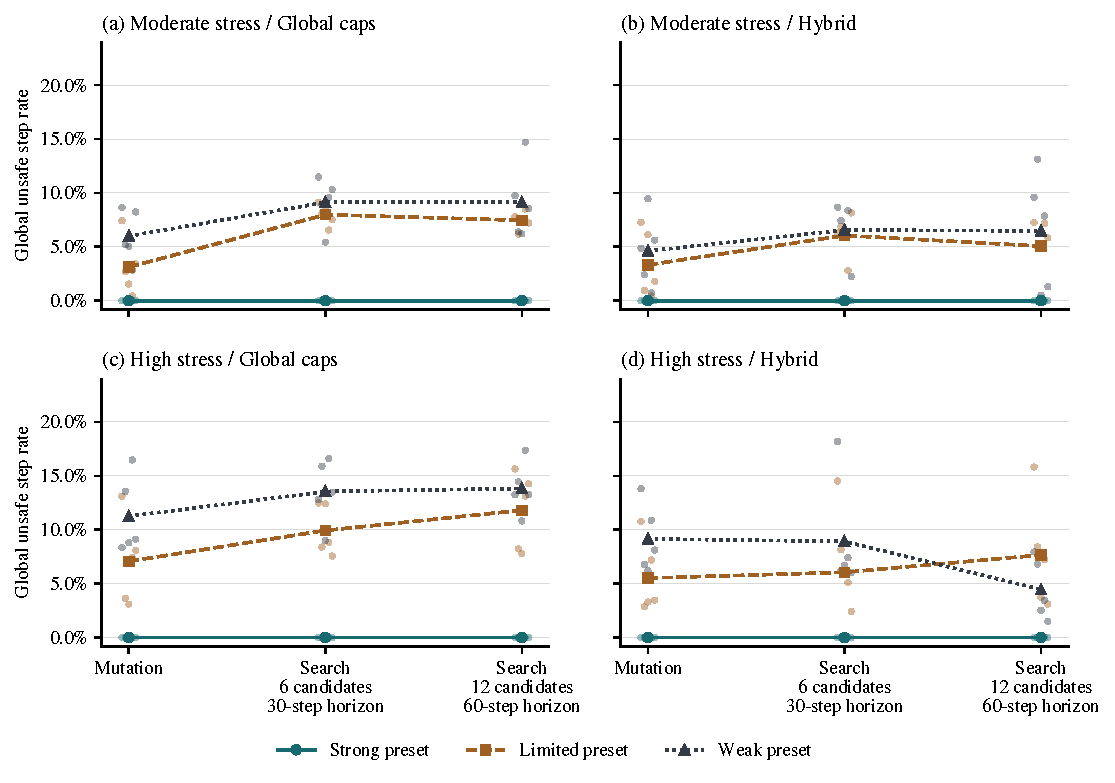
\includegraphics[width=\linewidth]{fig03_actor_factors}
\caption{Stage A with generation and oversight settings kept separate. Points are run values and lines are cell means. Bundled oversight presets still do not isolate recall, delay, capacity, and cost, and no common scalar capability scale is assumed.}
\end{figure}
\end{document}
